\documentclass{article}

\usepackage{setspace}
\usepackage{listings}
\usepackage{color}
\usepackage{xcolor}
\usepackage{geometry}
\usepackage{graphicx}
\usepackage{booktabs}
\usepackage[normalem]{ulem}
\usepackage{tabularx}
\usepackage{hyperref}
\usepackage{enumitem}
\usepackage{indentfirst}
\usepackage{biblatex}
\useunder{\uline}{\ul}{}
\usepackage{longtable}
\usepackage{color,colortbl}

\definecolor{Gray}{gray}{0.9}

\addbibresource{references.bib}

\geometry{a4paper,bindingoffset=0.2in,%
	left=1in,right=1in,top=1in,bottom=1in,%
	footskip=.25in}

\onehalfspacing

%opening
\title{MECHTRON 4TB6: Hazard Analysis \\ LifeLine}
\author{Group 30 \\ Emily Crowe, crowee \\ Arthur Faron, farona \\ Danushka Fernando, fernad12 \\Yerin Thevarajah, thevaryn \\ Phillip Truong, truonp1}

\begin{document}

\renewcommand{\labelenumii}{\arabic{enumi}.\arabic{enumii}}
\renewcommand{\labelenumiii}{\arabic{enumi}.\arabic{enumii}.\arabic{enumiii}}
\renewcommand{\labelenumiv}{\arabic{enumi}.\arabic{enumii}.\arabic{enumiii}.\arabic{enumiv}}

    \date{December 6, 2021}
	\maketitle
	
	\newpage
    
	\tableofcontents

	\newpage

	\section{Introduction}
	When designing a product it is of paramount importance to account for all potential behaviours of the system, both intended and not intended, and ensure that they meet or exceed all safety requirements. A thorough hazard analysis needs to be performed on the product to determine all the ways in which the device can malfunction, what impact the malfunction will have on the performance of the product, how it may affect the safety of the users, and what needs to be done to prevent the malfunction from occurring or to minimize its effect. This is especially important for a medical device such as the LifeLine which may be critical to the treatment and survival rate of the casualty. This document includes a comprehensive overview of all the components in the system, how the functionality of the device can be compromised, important safety considerations regarding the user and casualty, as well as a Failure Mode and Effects Analysis (FMEA) to determine potential system faults and their severity.
	
	\section{Definitions and Key Terms}
	\begin{itemize}
	    \item First responders: EMS, firefighters, paramedics, or police officers.
	    \item First aid:  Emergency care given to an individual in the case of serious injury with the aim to keep the individual alive and prevent further injury.
	    \item First-aider: Individual performing first aid.  For instance, a person trained in first aid arriving on a scene to treat an injured person.
	    \item Casualty: Individual receiving first aid treatment.
	    \item Vitals: The four vitals are body temperature, blood pressure, heart rate, and respiration rate. Vital signs are used to detect and monitor medical issues.  Lifeline will measure three vitals: body temperature, blood pressure, and heart rate.
	\end{itemize}
	
	\section{Background}
    The Portapres system by Finapres Medical Systems was a portable blood pressure monitoring device. It recorded finger arterial blood pressure, provided real-time visualization and could export data via serial port. A failure mode and effects analysis (FMEA) was performed on the existing device in hyperbaric conditions, and identified \cite{bg1}:
    \begin{itemize}
        \item Potential for spark formation from electrical components such as connections to battery supply and the carbon brush motorized pump
        \item Overheating due to increased power consumption
        \item Hyperbaric implosion hazard of the gas-filled electrolytic capacitors
    \end{itemize}
    This device has also been recalled through the FDA for reasons of the battery may become hot and leak \cite{bg2}.\\ \\
    The Apple watch was designed with electrocardiogram (ECG) and irregular heart rhythm features that were approved by the FDA. Those features provided continuous monitoring of ECG, data processing and analysis for the user. Though the FDA risk to health factors included \cite{bg3, bg4}:
    \begin{itemize}
        \item Poor quality ECG signal resulting in failure to detect arrhythmia 
        \item Misinterpretation and/or over-reliance on device output, leading to: Failure to seek treatment despite acute symptoms. Discontinuing or modifying treatment for chronic heart condition
        \item False negative resulting in failure to identify arrhythmia and delay of further evaluation or treatment
        \item False positive resulting in additional unnecessary medical procedures 

    \end{itemize}
    \section{Component Overview}
    
    \begin{figure}[!htb]
    	\centering
    	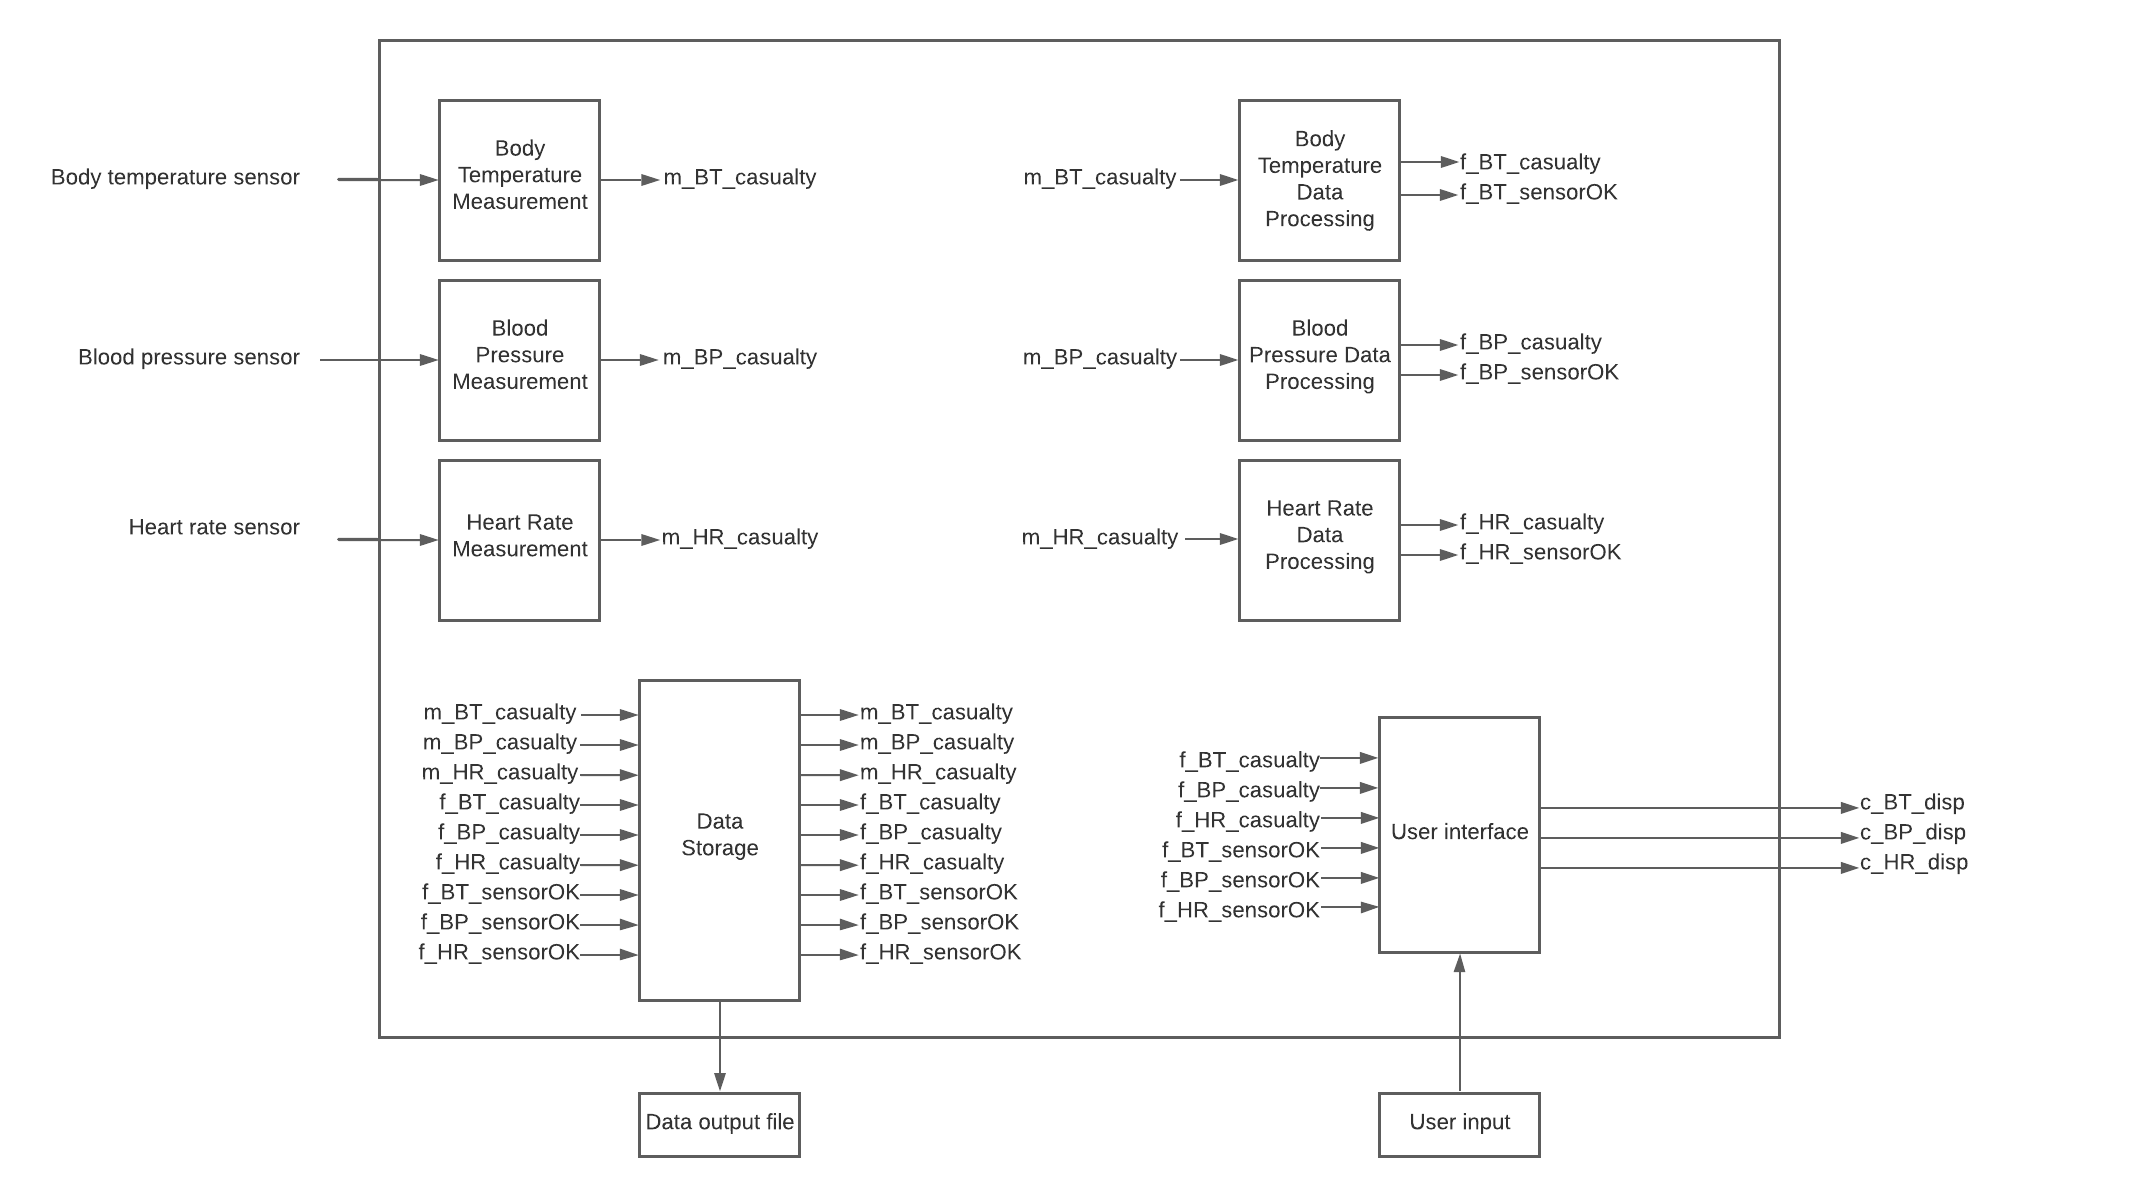
\includegraphics[width=1\linewidth]{f functions.png}
    	\caption{Component overview}
    \end{figure}
    
    \subsection{Components}
    \subsubsection{Body Temperature Measurement}
    The subsystem that measures a casualty's body temperature and passes it to the micro-controller. 
    \subsubsection{Blood Pressure Measurement}
    The subsystem that measures a casualty's blood pressure using a Pulse Express Pulse-Ox \& Heart Rate Sensor with MAX32664 and passes it to the micro-controller.
    \subsubsection{Heart Rate Measurement}
    The subsystem that measures a casualty's heart rate using a Pulse Express Pulse-Ox \& Heart Rate Sensor with MAX32664 and passes it to the micro-controller.
    \subsubsection{Body Temperature Data Processing}
    The subsystem that checks whether the body temperature is within a valid range.  If valid, the body temperature data is filtered and output to the display, otherwise the user is notified the data out of range. 
    \subsubsection{Blood Pressure Data Processing}
    The subsystem that checks whether the blood pressure data is within a valid range.  If valid, the blood pressure data is filtered and output to the display, otherwise the user is notified the data out of range.
    \subsubsection{Heart Rate Data Processing}
    The subsystem that checks whether the heart rate data is within a valid range.  If valid, the heart rate data is filtered and output to the display, otherwise the user is notified the data out of range.
    \subsubsection{Data Storage}
    The subsystem that stores the data from all three vitals (body temperature, blood pressure, and heart rate) before and after processing.  The data must be available after the device is powered off. 
    \subsubsection{Data Export}
    The subsystem that exports the data from the device's internal memory to an external device such as a USB memory drive or computer.  
    \subsubsection{User Interface}
    The subsystem contains two components: display and input.  The display must show the filtered vitals after processing.  The input must allow the user to give commands to delete or store data, export data, and switch between profiles for multiple casualties.  
    
    \section{Main Hazards to Casualty and User}
    \subsection{Casualty}
    \begin{enumerate}[label = (\alph*) ] 
        \item Electric shock
        \item Burns
        \item Misinterpretation of data by the user could lead to misdiagnosis
        \item Leaked medical data
    \end{enumerate}
    
    \subsection{User}
    \begin{enumerate}[label = (\alph*) ] 
        \item Electric shock
        \item Burns
    \end{enumerate}
    
    \section{Device Functionality Considerations}
    
    \subsection{Body Temperature Measurement}
        \subsubsection{Software} 
        \noindent
        None
        \subsubsection{Hardware}
        \begin{enumerate}[label = (\alph*) ] 
            \item Incorrect readings caused by faulty sensor or wiring.
            \item Ambient temperature is too cold or too hot for the sensor to operate correctly.
            \item Current and power ratings of body temperature sensor are exceeded.
            \item Motion artifact from casualty causes incorrect readings.
            \item Physical damage to the body temperature sensor causes incorrect readings.
            \item Body temperature sensor do not work and are unresponsive.
            \item Body temperature sensor reaches end-of-life and no longer functions correctly.
        \end{enumerate}
    \subsection{Blood Pressure Measurement}
        \subsubsection{Software}
        \noindent
        None
        \subsubsection{Hardware}
        \begin{enumerate}[label = (\alph*)]
            \item Incorrect readings caused by faulty sensor or wiring.
            \item Ambient temperature is too cold or too hot for the sensor to operate correctly.
            \item Current and power ratings of blood pressure sensor are exceeded.
            \item Motion artifact from casualty causes incorrect readings.
            \item Physical damage to the body temperature sensor causes incorrect readings.
            \item Blood pressure sensor does not work and is unresponsive.
            \item Blood pressure sensor reaches end-of-life and no longer functions correctly.
            \item Blood pressure readings are incorrect due to the limitations of PPG (photoplethysmogram).  For instance, nail polish needs to be removed.  
        \end{enumerate}
    
    \subsection{Heart Rate Measurement}
        \subsubsection{Software}
        \noindent
        None
        \subsubsection{Hardware}
        \begin{enumerate}[label = (\alph*)]
            \item Incorrect readings caused by faulty sensor or wiring.
            \item Ambient temperature is too cold or too hot for the sensor to operate correctly.
            \item Current and power ratings of heart rate sensor are exceeded.
            \item Motion artifact from casualty causes incorrect readings.
            \item Physical damage to the body temperature sensor causes incorrect readings.
            \item Heart rate sensor does not work and is unresponsive.
            \item Heart rate sensor reaches end-of-life and no longer functions correctly.
            \item Heart rate readings are incorrect due to the limitations of PPG (photoplethysmogram).  For instance, nail polish needs to be removed.
        \end{enumerate}
        
    \subsection{Body Temperature Data Processing}
        \subsubsection{Software}
        \begin{enumerate} [label = (\alph*)]
            \item Overflow errors cause incorrect readings or prevent the device from displaying the data completely.
            \item Calculation errors and rounding errors cause incorrect readings.
            \item Error within comparison between out-of-range values and measured data.
        \end{enumerate}
        \subsubsection{Hardware}
        \begin{enumerate} [label = (\alph*)]
            \item Analog LC filter parts malfunction.  For instance, capacitors and resistors short and cause incorrect values.
        \end{enumerate}
    
    
    \subsection{Blood Pressure Data Processing}
        \subsubsection{Software}
            \begin{enumerate} [label = (\alph*)]
                \item Overflow errors cause incorrect readings or prevent the device from displaying the data completely.
                \item Calculation errors and rounding errors cause incorrect readings.
                \item Error within comparison between out-of-range values and measured data.
            \end{enumerate}
        \subsubsection{Hardware}
            \begin{enumerate}[label = (\alph*)]
                \item Analog LC filter parts malfunction.  For instance, capacitors and resistors short and cause incorrect values.
            \end{enumerate}
    
    \subsection{Heart Rate Data Processing}
        \subsubsection{Software}
            \begin{enumerate}[label = (\alph*)]
                \item Overflow errors cause incorrect readings or prevent the device from displaying the data completely.
                \item Calculation errors and rounding errors cause incorrect readings.
                \item Error within comparison between out-of-range values and measured data. 
            \end{enumerate}
        \subsubsection{Hardware}
            \begin{enumerate}[label = (\alph*)]
                \item Analog LC filter parts malfunction.  For instance, capacitors and resistors short and cause incorrect values.
            \end{enumerate}
    
    \subsection{Data Storage and Export}
% Points that we thought of but need to expand or exclude: volatile/non volatile memory, device doesn't store data (immediately, power cycles), Incorrect Data (both input and output)

        \subsubsection{Software}
            \begin{enumerate}[label = (\alph*)]
                \item Encryption error causes a privacy breach of the casualty's medical data.
                \item Export file becomes corrupted.
                \item Overflow errors causes portions of data to be deleted.
                \item Volatile memory interrupted by accidental device shutdown results in loss of data.
            \end{enumerate}
        \subsubsection{Hardware}
            \begin{enumerate}[label = (\alph*)]
                \item Ambient temperature, either too hot or cold, affects device memory.
                \item Port malfunctions or physical damage to the port prevents it from operating properly.
            \end{enumerate}
    
    \subsection{User Interface}
        \subsubsection{Software}
            \begin{enumerate}[label = (\alph*)]
                \item Communication error between user input and micro-controller prevents user input from being picked up by the device. 
            \end{enumerate}
        \subsubsection{Hardware}
            \begin{enumerate}[label = (\alph*)]
                \item Overheating causes device to crash.
                \item Wire malfunction results in data displayed intermittently.
                \item If the touchscreen doesn't work or buttons are stuck, it prevents the first aider from switching between multiple patients, saving or deleting data, and exporting data. It could also affect the performance of the first aider as it will create a more stressful situation. 
                \item The screen malfunctions and stops working when the ambient temperature is too cold.  This too can affect the performance of the first aider.
                \item If the sunlight creates the issue of seeing the screen, this could affect the performance of the first aider. 
            \end{enumerate}
            
    \subsection{Micro-controller}
        \subsubsection{Software}
            \begin{enumerate}[label = (\alph*)]
                \item Unscheduled software updates results in the device being unable to record and save data. If this happens during an assessment out in the field, it could create a more stressful situation for the first aider.
            \end{enumerate}
        \subsubsection{Hardware}
            \begin{enumerate}[label = (\alph*)]
                \item  Ports of the micro-controller are faulty.
                \item  Wire issues between the micro-controller and its peripherals. 
            \end{enumerate}

    \subsection{Power}
        \subsubsection{Software}
            \begin{enumerate}[label = (\alph*)]
                \item  Device does not monitor the power supply level and inform the user of low battery.
            \end{enumerate}
        \subsubsection{Hardware}
            \begin{enumerate}[label = (\alph*)]
                \item  Battery leaks.   
                \item  Power supply degrades over time.
                \item  Ambient temperature affects the performance of the power supply.
                \item  Battery overheats.
            \end{enumerate}
    
    
    
    \section{Casualty and User Safety Considerations}
      
    \subsection{Casualty Applied Parts}
        \begin{enumerate}[label = (\alph*)]
            \item Current and power ratings are exceeded by device.
            \item Sensor overheats and burns casualty.
            \item Sensors placed on casualty's body shock the casualty electrically.
            \item Sensors induce medical shock from the casualty due to burning or electrical shock.
        \end{enumerate}
   
    \subsection{Data Privacy}
        \begin{enumerate}[label = (\alph*)]
            \item Encryption error causes a breach of casualty's private medical data.
        \end{enumerate}

    \subsection{Power Supply}
        \begin{enumerate}[label = (\alph*)]
            \item Casualty is not electrically isolated from the power supply.
            \item Battery leaks and acid corrodes casualty or user's skin.
            \item Battery enclosure is pierced causing it to combust.
            \item Battery overheats.
        \end{enumerate}
            
    \subsection{Misinterpretation of Data}
        \begin{enumerate}[label = (\alph*)]
            \item Over-reliance on device output causes user to not seek treatment even if it is required.
            \item False positive data results in prioritizing a casualty over others even if they are not in as much danger.    
        \end{enumerate}
        
    \subsection{Environment}
        \begin{enumerate}[label = (\alph*)]
            \item Device is wet.  
            \item Casualty is wet or lying on a conductive surface.
            \item Automated External Defibrillator (AED) damages device and poses risk to patient.
        \end{enumerate}

\newpage    
\section{FMEA Worksheet}

\begin{table}[!ht]
    \centering
    \begin{tabular}{|l|l|}
    \hline
        Scale & Severity \\ \hline
        0 & no impact  \\ \hline
        1 & low - some loss of functionality \\ \hline
        2 & moderately low - affects performance but not permanent \\ \hline
        3 & moderate - some permanent issue, poses no harm, device loses key functionality  \\ \hline
        4 & moderately high - device loses key functionality and there is harm to a person  \\ \hline
        5 & high impact - pose deadly harm to user or casualty  \\ \hline
    \end{tabular}
\end{table}

% Please add the following required packages to your document preamble:
% \usepackage{longtable}
% Note: It may be necessary to compile the document several times to get a multi-page table to line up properly
\begin{longtable}{|p{0.65\linewidth}|l|}
\hline
\textbf{Causes of Hazards}                               & \textbf{Severity}   \\
\endhead
%
                       & Out of 5   \\
\hline
\rowcolor{Gray}
Body Temperature Measurement                                       &                     \\
\hline
\textit{Hardware}                                                  &                     \\
\hline
6.1.2.a Incorrect readings caused by faulty sensor or wiring                                                                                                       & 3                   \\
\hline
6.1.2.b Ambient temperature is too cold or too hot for the sensor to operate correctly                                                                             & 2                   \\
\hline
6.1.2.c Current and power ratings of body temperature sensor are exceeded                                                                                          & 4                   \\
\hline
6.1.2.d Motion artifact from casualty causes incorrect readings                                                                                                    & 1                   \\
\hline
6.1.2.e Physical damage to the body temperature sensor causes incorrect readings                                                                                   & 3                   \\
\hline
6.1.2.f Body temperature sensor does not work and are unresponsive                                                                                                 & 3                   \\
\hline
6.1.2.g Body temperature sensor reaches end-of-life and no longer functions correctly                                                                              & 3                   \\
\hline 
\rowcolor{Gray}
Blood Pressure Measurement                                         &                     \\
\hline
\textit{Hardware}                                                  &                     \\
\hline
6.2.2.a Incorrect readings caused by faulty sensor or wiring                                                                                                        & 3                   \\
\hline
6.2.2.b Ambient temperature is too cold or too hot for the sensor to operate correctly                                                                             & 2                   \\
\hline
6.2.2.c Current and power ratings of blood pressure sensor are exceeded                                                                                            & 4                   \\
\hline
6.2.2.d Motion artifact from casualty causes incorrect readings                                                                                                    & 1                   \\
\hline
6.2.2.e Physical damage to the body temperature sensor causes incorrect readings                                                                                   & 3                   \\
\hline
6.2.2.f Blood pressure sensor does not work and is unresponsive.                                                                                                   & 3                   \\
\hline
6.2.2.g Blood pressure sensor reaches end-of-life and no longer functions correctly.                                                                               & 3                   \\
\hline
6.2.2.h Blood pressure readings are incorrect due to the limitations of PPG (photoplethysmogram).
For instance, nail polish needs to be removed.                   & 3                   \\
\hline   
\rowcolor{Gray}
Heart Rate Measurement                                             &                     \\
\hline
\textit{Hardware}                                                  &                     \\
\hline
6.3.2.a Incorrect readings caused by faulty sensor or wiring     & 3                   \\
\hline
6.3.2.b Ambient temperature is too cold or too hot for the sensor to operate correctly                                                                             & 2                   \\
\hline
6.3.2.c Current and power ratings of heart rate sensor are exceeded.                                                                                               & 4                   \\
\hline
6.3.2.d Motion artifact from casualty causes incorrect readings. & 1                   \\
\hline
6.3.2.e Physical damage to the body temperature sensor causes incorrect readings.                                                                                  & 3                   \\
\hline
6.3.2.f Heart rate sensor does not work and is unresponsive.     & 3                   \\
\hline
6.3.2.g Heart rate sensor reaches end-of-life and no longer functions correctly.                                                                                   & 3                   \\
\hline
6.3.2.h Heart rate readings are incorrect due to the limitations of PPG (photoplethysmogram). For
instance, nail polish needs to be removed.                       & 3                   \\
\hline 
\rowcolor{Gray}
Body Temperature Data Processing                                   &                     \\
\hline
\textit{Software}                                                  &                     \\
\hline
6.4.1.a Overflow errors cause incorrect readings or prevent the device from displaying the data completely.                                                      & 3                   \\
\hline
6.4.1.b Calculation errors and rounding errors cause incorrect readings.                                                                                           & 3                   \\
\hline
6.4.1.c Error within comparison between out-of-range values and measured data.                                                                                     & 3                   \\
\hline
\textit{Hardware}                                                  &                     \\
\hline
6.4.2.a Analog LC filter parts malfunction. For instance, capacitors and resistors short and cause
incorrect values.                                                & 3                   \\
\hline    
\rowcolor{Gray}
Blood Pressure Data Processing                                     &                     \\
\hline
\textit{Software}                                                  &                     \\
\hline
6.5.1.a Overflow errors cause incorrect readings or prevent the device from displaying the data completely.                                                 & 3                   \\
\hline
6.5.1.b Calculation errors and rounding errors cause incorrect readings.                                                                                           & 3                   \\
\hline
6.5.1.c Error within comparison between out-of-range values and measured data.                                                                                     & 3                   \\
\hline
\textit{Hardware}                                                &                     \\
\hline
6.5.2.a Analog LC filter parts malfunction. For instance, capacitors and resistors short and cause
incorrect values.                                                & 3                   \\
\hline    
\rowcolor{Gray}
Heart Rate Data Processing                                         &                     \\
\hline
\textit{Software}                                                  &                     \\
\hline
6.6.1.a Overflow errors cause incorrect readings or prevent the device from displaying the data completely.                                                      & 3                   \\
\hline
6.6.1.b Calculation errors and rounding errors cause incorrect readings                                                                                            & 3                   \\
\hline
6.6.1.c Error within comparison between out-of-range values and measured data.                                                                                     & 3                   \\
\hline
\textit{Hardware}                                                  &                     \\
\hline
6.6.2.a Analog LC filter parts malfunction. For instance, capacitors and resistors short and cause
incorrect values                                                 & 3                   \\
\hline
\rowcolor{Gray}
Data Storage and Export                                            &                    \\
\hline
\textit{Software}                                                  &                     \\
\hline
6.7.1.a Encryption error causes a privacy breach of the casualty’s medical data                                                                                    & 4                   \\
\hline
6.7.1.b Export file becomes corrupted                            & 3                   \\
\hline
6.7.1.c Overflow errors causes portions of data to be deleted.                                                                                                   & 3                   \\
\hline
6.7.1.d Volatile memory interrupted by accidental device shutdown results in loss of data                                                                        & 3                   \\
\hline
\textit{Hardware}                                                  &                     \\
\hline
6.7.2.a Ambient temperature, either too hot or cold, affects device memory.                                                                                   & 3                   \\
\hline
6.7.2.b Port malfunctions or physical damage to the port prevents it from operating properly.                                                                  & 3                   \\
\hline 
\rowcolor{Gray}
User Interface                                                     &                     \\
\hline
\textit{Software}                                                  &                     \\
\hline
6.8.1.a Communication error between user input and micro-controller prevents user input from being
picked up by the device.                                         & 2                   \\
\hline
\textit{Hardware}                                                  &                     \\
\hline
6.8.2.a Overheating causes device to crash                       & 2                   \\
\hline
6.8.2.b Wire malfunction results in data displayed intermittently.                                                                                            & 1                   \\
\hline
6.8.2.c If the touchscreen doesn’t work or buttons are stuck, it prevents the first aider from switching between multiple patients, saving or deleting data, and exporting data. It could also affect the performance of the first aider as it will create a more stressful situation                                                                             & 2                   \\
\hline
6.8.2.d The screen malfunctions and stops working when the ambient temperature is too cold. This
too can affect the performance of the first aider.
                                                                & 2                   \\
\hline
6.8.2.e If the sunlight creates the issue of seeing the screen, this could affect the performance of the first aider.                                              & 1                   \\
\hline  
\rowcolor{Gray}
Micro-controller                                                   &                     \\
\hline
\textit{Software}                                                  &                     \\
6.9.1.a Unscheduled software updates results in the device being unable to record and save data. If this happens during an assessment out in the field, it could create a more stressful situation for the first aider.                                             & 3                   \\
\hline
\textit{Hardware}                                                  &                     \\
\hline
6.9.2.a Ports of the micro-controller are faulty.
                                                                 & 2                  \\
\hline
6.9.2.b Wire issues between the micro-controller and its peripherals.                                                                                             & 2                   \\
\hline   
\rowcolor{Gray}
Power                                                              &                     \\
\hline
\textit{Software}                                                  &                     \\
\hline
6.10.1.a Device does not monitor the power supply level and inform the user of low battery.                                                                        & 3                   \\
\hline
\textit{Hardware}                                                  &                     \\
\hline
6.10.2.a Battery leaks.                                          & 4                   \\
\hline
6.10.2.b Power supply degrades over time                         & 1                   \\
\hline
6.10.2.c Ambient temperature affects the performance of the power supply.                                                                                          & 1                   \\
\hline
6.10.2.d Battery overheats.                                      & 3                   \\
\hline
\rowcolor{Gray}
Casualty Applied Parts                                            &                     \\
\hline
7.1.a Current and power ratings are exceeded by device.                                                                                                            & 4                   \\
\hline
7.1.b Sensor overheats and burns casualty.                       & 4                   \\
\hline
7.1.c Sensors placed on casualty’s body shock the casualty electrically.                                                                                           & 4                   \\
\hline
7.1.d Sensors induce medical shock from the casualty due to burning or electrical shock.                                                                           & 4                   \\
\hline
\rowcolor{Gray}
Data Privacy                                                       &                     \\
\hline
7.2.a Encryption error causes a breach of casualty’s private medical data                                                                                          & 4                   \\
\hline
\rowcolor{Gray}
Power Supply                                                       &                     \\
\hline
7.3.a Casualty is not electrically isolated from the power supply                                                                                                  & 4                   \\
\hline
7.3.b Battery leaks and acid corrodes casualty or user’s skin.                                                                                                     & 4                   \\
\hline
7.3.c Battery enclosure is pierced causing it to combust.                                                                                                          & 4                   \\
\hline
7.3.d Battery overheats.                                         & 4                   \\
\hline
\rowcolor{Gray}
Misinterpretation of Data                                          &                     \\
\hline
7.4.a Over-reliance on device output causes user to not seek treatment even if it is required.                                                                     & 3                   \\
\hline
7.4.b False positive data results in prioritizing a casualty over others even if they are not in as much danger                                                   & 4                   \\
\hline
\rowcolor{Gray}
Environment                                                        &                     \\
\hline
7.5.a Device is wet                                              & 3                   \\
\hline
7.5.b Casualty is wet or lying on a conductive surface.                                                                                                            & 2                   \\
\hline
7.5.c Automated External Defibrillator (AED) damages device and poses risk to patient.                                                                             & 4                  \\
\hline
\end{longtable}
\newpage
\section{Roadmap}

\begin{figure}[!htb]
    	\centering
    	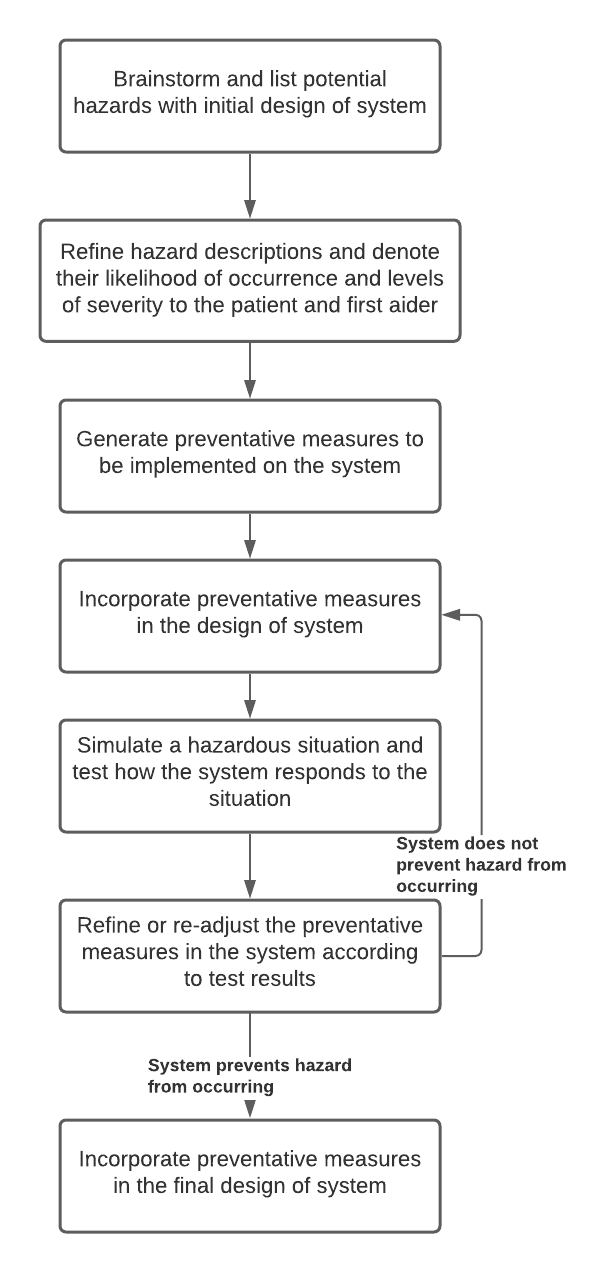
\includegraphics[width=0.60\linewidth]{hazard analysis - roadmap.png}
    	\caption{The iterative process of hazard analysis}
    	\label{flowchart}
    \end{figure}
    
\newpage
\section{Appendix}
	\printbibliography

\end{document}
